% !Mode:: "TeX:UTF-8"
\chapter{Practice: Stereo Visual SLAM}
\begin{mdframed}  
	\textbf{Goal of Study}
	\begin{enumerate}[labelindent=0em,leftmargin=1.5em]
	\item Implement a stereo visual SLAM from scratch.
	\item Understand the problems that are prone to occur in VO and how to fix them.
	\end{enumerate}
\end{mdframed}

This lecture is the concluding part of the book. We will use the knowledge we learned before to actually write a visual odometry program. You will manage local robot trajectories and landmarks and experience how a software framework is composed. During the operation, we will encounter many practical problems: how to continuously track the image, control the scale of BA, and so on. To make the program run stably, we need to deal with the above situations, which will bring about many useful discussions on engineering realization.

\newpage
\section{Why do We Have a Separate Engineering Chapter?}
Knowing the principles of bricks and cement does not mean that you can build a grand palace.

In the Minecraft game, all the players have are some blocks with different colors and textures. All the player needs to do is place these blocks on a plane and stack them together. Understanding a block is also extremely simple, but most beginners can only make simple matchbox houses when really starting to build the architectures. Experienced and creative players can use these simple blocks to build houses, gardens, terraces, and pavilions, even the big cities (\autoref{fig:mcarchitecture}~) \footnote{The lower left is my practice work. The bottom right is from the work of the Epicwork team: "Old Summer Palace." I used to study in Epicwork for a while. The creativity of the young people and even the children there left a deep impression on me. }.

\begin{figure}[!htp]
	\centering    
	\includegraphics[width=0.9\linewidth]{designVO/mcarchitecture}\\
	\caption{Great work normally starts from simple things.}
	\label{fig:mcarchitecture}
\end{figure}

In SLAM, we believe that engineering implementation and understanding of algorithm principles should be at least the same important, or even more, as the algorithm principles. The algorithms are like blocks in the building. We can discuss their properties clearly, but just understanding the basic units will not enable you to build an entire building. They require a lot of trials, time, and experience. We encourage readers to work in a more practical direction. Of course, this is often very complicated. Just like in Minecraft, you need to master the structure of various columns, walls, and roofs, wall carvings, and calculation of geometric angles. There are far more contents than discussing the nature of each block.

The same is true for the specific implementation of SLAM. A practical program has a lot of engineering design and skills (tricks), and it is necessary to discuss how to deal with problems after each step. In principle, each SLAM implementation is different. Most of the time, we cannot say which implementation method is the best. However, we usually encounter some common problems like managing map points, dealing with mismatches, selecting keyframes, and so on. We hope that readers can have some intuitive feelings about these possible problems. We think this feeling is vital.

Therefore, out of the emphasis on practice, in this lecture, we will lead the readers through the process of building a SLAM framework. Just like the architecture, we have to discuss trivial but essential issues such as column spacing and facade aspect ratio. SLAM engineering is complicated. Even if we only keep the core part, it will take up a lot of space and make this book too verbose. However, please note that although the final completed project may be complicated, the process of being simple to complex is worthy of detailed discussion. Therefore, we have to start from a simple data structure first, make simple visual odometry, and then slowly add some additional functions. 

The code for this lecture is in \textit{slambook2/ch13}. We will implement a simplified version of stereo VO and then see its running effect in the Kitti dataset. This VO consists of a frontend of optical flow tracking and a backend of sliding window BA. Why choose stereo VO? One reason is that the stereo vision is relatively simple to implement, and initialization can be completed in a single frame. The second is that the stereo camera has 3D observation, and the realization effect will be better than that of the monocular.

\section{Framework}
We are discussing a project realization, and the project usually has the concept of a framework. Most Linux libraries will classify and store algorithm code files according to modules. For example, the header files will be placed in the header file directory, and the source code will be placed in the source code directory. Also, there may be configuration files, test files, third-party libraries, and so on. Now we come to classify our files according to the common practice of small algorithm libraries:

\begin{enumerate}
	\item \textit{bin} stores the compiled binary file;
	\item \textit{include/myslam} stores the header files of the SLAM module. 
	\item \textit{src} stores the source code files, mainly .cpp files.
	\item \textit{test} stores the files used for testing, which are also .cpp files.
	\item \textit{config} stores the configuration files.
	\item \textit{cmake\_modules} saves the cmake files of third-party libraries, which are used by libraries such as g2o.
\end{enumerate}

In this way, we have determined the location of the code file. Now let's discuss the basic data structure involved in VO.

\subsection{Data Structure}
Before writing code, we should be clear about what we want to write. A long time ago, there was an old view that a program is \textbf{data structure+algorithm}, so for VO, we have to ask: What kind of data does VO need to process? What are the key algorithms involved? What is the relationship between them?

After simple thinking, we can easily conclude:
\begin{itemize}
	\item The most basic unit we deal with is \textbf{image}. In stereo VO, that is \textbf{a pair of images}, we might as well call it a \textbf{frame}.
	\item We will mention \textbf{features} for the frame. These features are many 2D points.
	\item We look for the association of features between images. If you can see a feature multiple times, you can use the triangulation method to calculate its 3D position, that is, \textbf{landmarks}.
\end{itemize}

Obviously, \textbf{image}, \textbf{features}, and \textbf{landmarks} are the most basic structures in our system. The relationship between them is shown in \autoref{fig:frame-feature-landmark}. In the following description, \textbf{landmarks} and \textbf{map points} refer to points in 3D space, and their semantics are the same.

\begin{figure}[!htp]
	\centering
	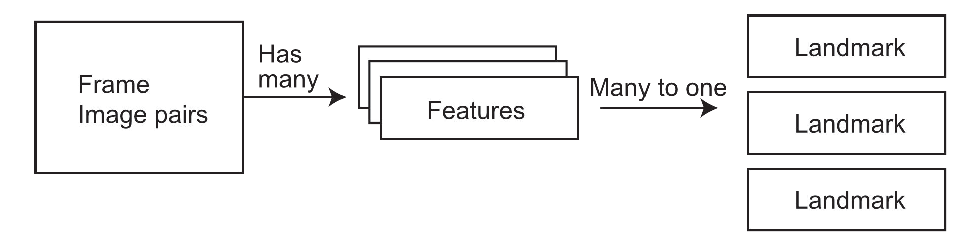
\includegraphics[width=1.0\linewidth]{designVO/frame-feature-landmark.pdf}
	\caption{Basic data structure and their relationships.}
	\label{fig:frame-feature-landmark}
\end{figure}

\subsection{Pipeline}
Well, next we have to ask, which algorithms are responsible for feature extraction, which algorithms are responsible for triangulation, and which algorithms are there to deal with optimization problems? According to the previous introduction in this book, we believe that SLAM consists of front and backends. The frontend is responsible for calculating the feature matching of adjacent images, and the backend is responsible for optimizing the entire problem. In a typical implementation, the two should have their own threads. The frontend fast processing ensures real-time performance, and the backend optimizes keyframes to ensure good results. So overall, our program has two important modules:

\begin{itemize}
	\item Frontend. We insert an image frame into the frontend, and the frontend is responsible for extracting the features in the image, and then perform optical flow tracking with the previous frame, and calculate the position of the frame based on the optical flow result. When necessary, new feature points should be added and triangulated. The result of the frontend processing will be used as the initial value of the backend optimization.
	\item Backend. The backend is a slower thread. It gets the processed keyframes and landmark points, optimizes them, and then returns the optimized results. The backend should control the scale of the optimization problem within a certain range and cannot keep growing over time.
\end{itemize}

Through this analysis, we can determine the framework of the entire algorithm, and then express it in a popular pipeline diagram, such as \autoref{fig:pipeline}. We put a \textbf{map} module between the front and backends to handle the data flow between them. Since the front and backends process data in separate threads, our envisioned process should be to add new data to the map after the frontend has extracted the keyframes; when the backend detects that the map is updated, it runs an optimization, and then puts the old in the map. The keyframes and map points are removed to maintain the optimized scale.

\begin{figure}[!htp]
	\centering
	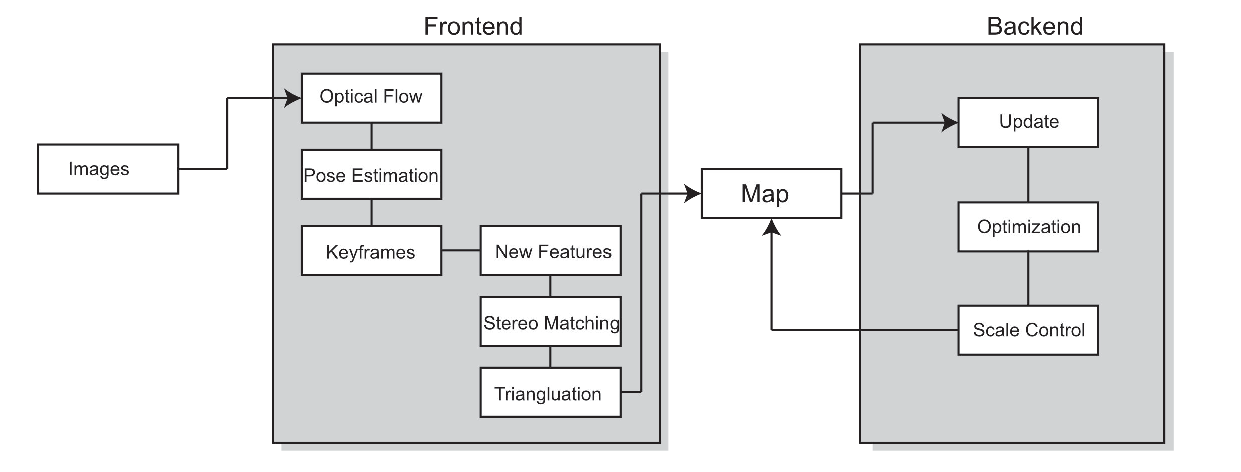
\includegraphics[width=1.0\linewidth]{designVO/pipeline.pdf}
	\caption{Processing pipeline.}
	\label{fig:pipeline}
\end{figure}

In this way, we have determined the general system flow, which will help the subsequent coding realization. Of course, in addition to the core algorithm, we also need some small peripheral modules to make the system more convenient, such as:
\begin{itemize}
	\item We should have a camera class to manage the internal and external parameters and projection functions of the camera.
	\item We need a configuration file management class to facilitate reading content from configuration files. Some important parameters can be recorded in the configuration file to facilitate our adjustment;
	\item Because the final algorithm runs on the Kitti dataset, we need to read the image data according to Kitti's storage format, which should also be handled by a separate class.
	\item We need a visualization module to observe the running status of the system, otherwise we have to scratch our heads against a series of values。
\end{itemize}

Although these modules are not the core, they are indispensable. Due to space limitations, we leave the peripheral code to readers to read by themselves, and only the core parts are introduced in the book.

\section{Implementation}
\subsection{Implement the Basic Data Structure}
Based on the discussion in the previous lecture, let's first implement the three categories of frame, feature, and landmark. For basic data structures, it is usually recommended to set them as \textit{structs} without the need to define complex private variables and interfaces. Considering that these data may be accessed and modified by multiple threads, we need to add thread locks in key parts.

We write the frame \textit{struct} as:
\begin{lstlisting}[language=c++,caption=slambook2/ch13/include/myslam/frame.h]
struct Frame {
public:
	EIGEN_MAKE_ALIGNED_OPERATOR_NEW;
	typedef std::shared_ptr<Frame> Ptr;
	
	unsigned long id_ = 0;           // id of this frame
	unsigned long keyframe_id_ = 0;  // id of keyframe
	bool is_keyframe_ = false;       // keyframe?
	double time_stamp_;              // timestamp, not used in Kitti
	SE3 pose_;                       // pose defined as Tcw
	std::mutex pose_mutex_;          // Pose data mutex
	cv::Mat left_img_, right_img_;   // stereo images
	
	// extracted features in left image
	std::vector<std::shared_ptr<Feature>> features_left_;
	// corresponding features in right image, set to nullptr if no corresponding
	std::vector<std::shared_ptr<Feature>> features_right_;
	
	public:  // data members
	Frame() {}
	
	Frame(long id, double time_stamp, const SE3 &pose, const Mat &left,
	const Mat &right);
	
	// set and get pose, thread safe
	SE3 Pose() {
		std::unique_lock<std::mutex> lck(pose_mutex_);
		return pose_;
	}
	
	void SetPose(const SE3 &pose) {
		std::unique_lock<std::mutex> lck(pose_mutex_);
		pose_ = pose;
	}
	
	/// Set keyframe and keyframe_id 
	void SetKeyFrame();
	
	/// create new frame and allocate id
	static std::shared_ptr<Frame> CreateFrame();
};
\end{lstlisting}

We define Frame to contain id, pose, image, and features in the left and right images. Among them, Pose will be set or accessed by the front and backends at the same time, so we define its set and get functions, and lock the data in the function. At the same time, Frame can be constructed by static functions, and its id can be automatically assigned in static functions.

Next, the feature struct:
\begin{lstlisting}[language=c++,caption=slambook2/ch13/include/myslam/feature.h]
struct Feature {
	EIGEN_MAKE_ALIGNED_OPERATOR_NEW;
	typedef std::shared_ptr<Feature> Ptr;
	
	std::weak_ptr<Frame> frame_;         // the frame that takes this feature
	cv::KeyPoint position_;              // 2D pixel position
	std::weak_ptr<MapPoint> map_point_;  // assigned map point
	
	bool is_outlier_ = false;       // is outlier?
	bool is_on_left_image_ = true;  // is detected on the left image?
	
	Feature() {}
	
	Feature(std::shared_ptr<Frame> frame, const cv::KeyPoint &kp)
		: frame_(frame), position_(kp) {}
};
\end{lstlisting}

The main information of Feature is its 2D position and several flags describing whether it is an abnormal point and whether it is extracted in the left camera. We can access the Frame holding it and its corresponding map point through a Feature object. However, the actual ownership rights of Frame and MapPoint belong to the map. In order to avoid the circular reference generated by shared\_ptr \footnote{In short, Frame holds the shared\_ptr of Feature, so you should avoid Feature holding Frame's  shared\_ptr again, otherwise the two struct refer to each other, which will cause the smart pointer to fail to be automatically destructed. }, weak\_ptr is used here.

Finally the map point, or landmark:
\begin{lstlisting}[language=c++,caption=slambook2/ch13/include/myslam/mappoint.h]
struct MapPoint {
	EIGEN_MAKE_ALIGNED_OPERATOR_NEW;
	typedef std::shared_ptr<MapPoint> Ptr;
	unsigned long id_ = 0;  // ID
	bool is_outlier_ = false;
	Vec3 pos_ = Vec3::Zero();  // Position in world
	std::mutex data_mutex_;
	int observed_times_ = 0;  // being observed by feature matching algo.
	std::list<std::weak_ptr<Feature>> observations_;
	
	MapPoint() {}
	
	MapPoint(long id, Vec3 position);
	
	Vec3 Pos() {
		std::unique_lock<std::mutex> lck(data_mutex_);
		return pos_;
	}
	
	void SetPos(const Vec3 &pos) {
		std::unique_lock<std::mutex> lck(data_mutex_);
		pos_ = pos;
	};
	
	void AddObservation(std::shared_ptr<Feature> feature) {
		std::unique_lock<std::mutex> lck(data_mutex_);
		observations_.push_back(feature);
		observed_times_++;
	}
	
	void RemoveObservation(std::shared_ptr<Feature> feat);
	
	std::list<std::weak_ptr<Feature>> GetObs() {
		std::unique_lock<std::mutex> lck(data_mutex_);
		return observations_;
	}
	
	// factory function
	static MapPoint::Ptr CreateNewMappoint();
};
\end{lstlisting}

The most important thing about MapPoint is its 3D position, which is the pos\_ variable, also needs to be locked. Its observation\_ variable records the features that observed this map point. Because Feature may be judged as outlier, it needs to be locked when the observation part is changed.

So far we have realized the basic data structure. In the framework, we let the map class actually hold these Frame and MapPoint objects, so we also need to define a map class:

\begin{lstlisting}[language=c++,caption=slambook2/ch13/include/myslam/map.h]
class Map {
	public:
	EIGEN_MAKE_ALIGNED_OPERATOR_NEW;
	typedef std::shared_ptr<Map> Ptr;
	typedef std::unordered_map<unsigned long, MapPoint::Ptr> LandmarksType;
	typedef std::unordered_map<unsigned long, Frame::Ptr> KeyframesType;
	
	Map() {}
	
	void InsertKeyFrame(Frame::Ptr frame);
	
	void InsertMapPoint(MapPoint::Ptr map_point);
	
	LandmarksType GetAllMapPoints() {
		std::unique_lock<std::mutex> lck(data_mutex_);
		return landmarks_;
	}

	KeyframesType GetAllKeyFrames() {
		std::unique_lock<std::mutex> lck(data_mutex_);
		return keyframes_;
	}
	
	LandmarksType GetActiveMapPoints() {
		std::unique_lock<std::mutex> lck(data_mutex_);
		return active_landmarks_;
	}
	
	KeyframesType GetActiveKeyFrames() {
		std::unique_lock<std::mutex> lck(data_mutex_);
		return active_keyframes_;
	}
	
	void CleanMap();
	
	private:

	void RemoveOldKeyframe();
	
	std::mutex data_mutex_;
	LandmarksType landmarks_;         // all landmarks
	LandmarksType active_landmarks_;  // active landmarks
	KeyframesType keyframes_;         // all keyframes
	KeyframesType active_keyframes_;  // all keyframes
	
	Frame::Ptr current_frame_ = nullptr;
	
	// settings
	int num_active_keyframes_ = 7;  
};
\end{lstlisting}

The map records all keyframes and corresponding landmark in a hash form, and maintains an activated keyframe and map point at the same time. Here the concept of \textbf{activation} is what we call \textbf{sliding window}, which will move forward over time. The backend will extract the activated keyframes and landmark points from the map for optimization, and ignore the rest to achieve the effect of controlling the optimization scale. Of course, the activation strategy is defined by ourselves. The simple activation strategy is to remove the oldest keyframe and keep the latest keyframes in time. We only keep the latest 7 keyframes in this demo.

\subsection{Implement the Frontend}
After defining the basic data structure, let's consider the frontend functions. The frontend needs to determine the pose of the frame based on the binocular image, but there are some different methods in actual implementation. For example, how should we use the right-hand image? Does it compare each frame with the left and right eye, or just compare one of the left and right eye? When we triangulate, should we consider the triangulation of the left and right images, or should we consider the triangulation of the front and back frames in time? In fact, any two images can be triangulated (for example, the left image of the previous frame vs. the right image of the next frame), so everyone's realization will be different.

For simplicity, we first determine the frontend processing logic:
\begin{enumerate}
	\item The frontend has three states: \textbf{initialization}, \textbf{normal tracking}, and \textbf{tracking lost}.
	\item In the initialization state, according to the optical flow matching between the left and right eyes, find the map points that can be triangulated, and establish the initial map when successful.
	\item In the tracking phase, the frontend calculates the optical flow from the feature point of the previous frame to the current frame, and calculates the image pose based on the optical flow result. This calculation uses only the left eye image, not the right eye.
	\item If fewer points are tracked, the current frame is judged to be a keyframe. For keyframes, do the following things:
	
	\begin{itemize}
		\item Extract new feature points;
		\item Find the corresponding points of these points on the right, and use triangulation to create new landmarks;
		\item Add new keyframes and landmarks to the map and trigger a backend optimization.
		\item If the tracking is lost, reset the frontend system and reinitialize it.
	\end{itemize}
\end{enumerate}

According to this logic, the frontend processing flow is roughly as follows:
\begin{lstlisting}[language=c++,caption=slambook2/ch13/src/frontend.cpp]
bool Frontend::AddFrame(myslam::Frame::Ptr frame) {
	current_frame_ = frame;
	switch (status_) {
		case FrontendStatus::INITING:
			StereoInit();
			break;
		case FrontendStatus::TRACKING_GOOD:
		case FrontendStatus::TRACKING_BAD:
			Track();
			break;
		case FrontendStatus::LOST:
			Reset();
			break;
	}
	
	last_frame_ = current_frame_;
	return true;
}
\end{lstlisting}

The Track() is implemented as:
\begin{lstlisting}[language=c++,caption=slambook2/ch13/src/frontend.cpp]
bool Frontend::Track() {
	if (last_frame_) {
		current_frame_->SetPose(relative_motion_ * last_frame_->Pose());
	}
	
	int num_track_last = TrackLastFrame();
	tracking_inliers_ = EstimateCurrentPose();
	
	if (tracking_inliers_ > num_features_tracking_) {
		// tracking good
		status_ = FrontendStatus::TRACKING_GOOD;
	} else if (tracking_inliers_ > num_features_tracking_bad_) {
		// tracking bad
		status_ = FrontendStatus::TRACKING_BAD;
	} else {
		// lost
		status_ = FrontendStatus::LOST;
	}
	
	InsertKeyframe();
	relative_motion_ = current_frame_->Pose() * last_frame_->Pose().inverse();
	
	if (viewer_) viewer_->AddCurrentFrame(current_frame_);
	return true;
}
\end{lstlisting}

In the TrackLastFrame(), we call the optical flow of OpenCV to track the feature points:
\begin{lstlisting}[language=c++,caption=slambook2/ch13/src/frontend.cpp]
int Frontend::TrackLastFrame() {
	// use LK flow to estimate points in the right image
	std::vector<cv::Point2f> kps_last, kps_current;
	for (auto &kp : last_frame_->features_left_) {
		if (kp->map_point_.lock()) {
			// use project point
			auto mp = kp->map_point_.lock();
			auto px =
			camera_left_->world2pixel(mp->pos_, current_frame_->Pose());
			kps_last.push_back(kp->position_.pt);
			kps_current.push_back(cv::Point2f(px[0], px[1]));
		} else {
			kps_last.push_back(kp->position_.pt);
			kps_current.push_back(kp->position_.pt);
		}
	}
	
	std::vector<uchar> status;
	Mat error;
	cv::calcOpticalFlowPyrLK(
	last_frame_->left_img_, current_frame_->left_img_, kps_last,
	kps_current, status, error, cv::Size(21, 21), 3,
	cv::TermCriteria(cv::TermCriteria::COUNT + cv::TermCriteria::EPS, 30, 0.01),
	cv::OPTFLOW_USE_INITIAL_FLOW);
	
	int num_good_pts = 0;
	
	for (size_t i = 0; i < status.size(); ++i) {
		if (status[i]) {
			cv::KeyPoint kp(kps_current[i], 7);
			Feature::Ptr feature(new Feature(current_frame_, kp));
			feature->map_point_ = last_frame_->features_left_[i]->map_point_;
			current_frame_->features_left_.push_back(feature);
			num_good_pts++;
		}
	}
	
	LOG(INFO) << "Find " << num_good_pts << " in the last image.";
	return num_good_pts;
}
\end{lstlisting}

In the implementation, we often split the complex functions into some short functions, until the underlying functions call OpenCV or g2o to achieve specific calculation. In this way, the readability and reusability of the program can be improved. For example, the same feature extraction function can be used for initialization phase and the new feature detection part of the keyframe. We recommend that readers go through this code by yourself (in fact, the frontend is less than 400 lines of code).

\subsection{Implement the Backend}
Compared with the frontend, the logic of the backend implementation will be more complicated. The overall backend implementation is as follows:
\begin{lstlisting}[language=c++,caption=slambook2/ch13/include/myslam/backend.h]
class Backend {
public:
	EIGEN_MAKE_ALIGNED_OPERATOR_NEW;
	typedef std::shared_ptr<Backend> Ptr;
	
	/// Start the backend thread in the constructor 
	Backend();
	
	// Set cameras and fetch the params
	void SetCameras(Camera::Ptr left, Camera::Ptr right) {
		cam_left_ = left;
		cam_right_ = right;
	}

	void SetMap(std::shared_ptr<Map> map) { map_ = map; }
	
	/// optimize and update the map
	void UpdateMap();
	
	/// stop the backend
	void Stop();
	
private:
	/// backend thread
	void BackendLoop();
	
	/// optimize the sliding window
	void Optimize(Map::KeyframesType& keyframes, Map::LandmarksType& landmarks);
	
	std::shared_ptr<Map> map_;
	std::thread backend_thread_;
	std::mutex data_mutex_;
	
	std::condition_variable map_update_;
	std::atomic<bool> backend_running_;
	
	Camera::Ptr cam_left_ = nullptr, cam_right_ = nullptr;
};
\end{lstlisting}

Finally, we look at the running effect of this visual odometry. First we need to download the Kitti dataset from: \url{http://www.cvlibs.net/datasets/kitti/eval_odometry.php}. Its odometry data is about 22GB. After downloading, we decompress it and get several video segments. Let's take segment 0 as an example. After compiling the program in this section, fill in the path corresponding to the data in the configuration file config/default.yaml. In my machine it looks like:
$$\text{dataset_dir: /media/xiang/Data/Dataset/Kitti/dataset/sequences/00}.$$

Then we run it with:
\begin{lstlisting}[language=sh,caption=Terminal input:]
	bin/run_kitti_stereo
\end{lstlisting}
Then you can see the positioning output, as shown in \autoref{fig:snapshot-vo}. During operation, the program will display the activated keyframes and maps, which should continue to grow and disappear as the camera moves.

\begin{figure}[!htp]
	\centering    
	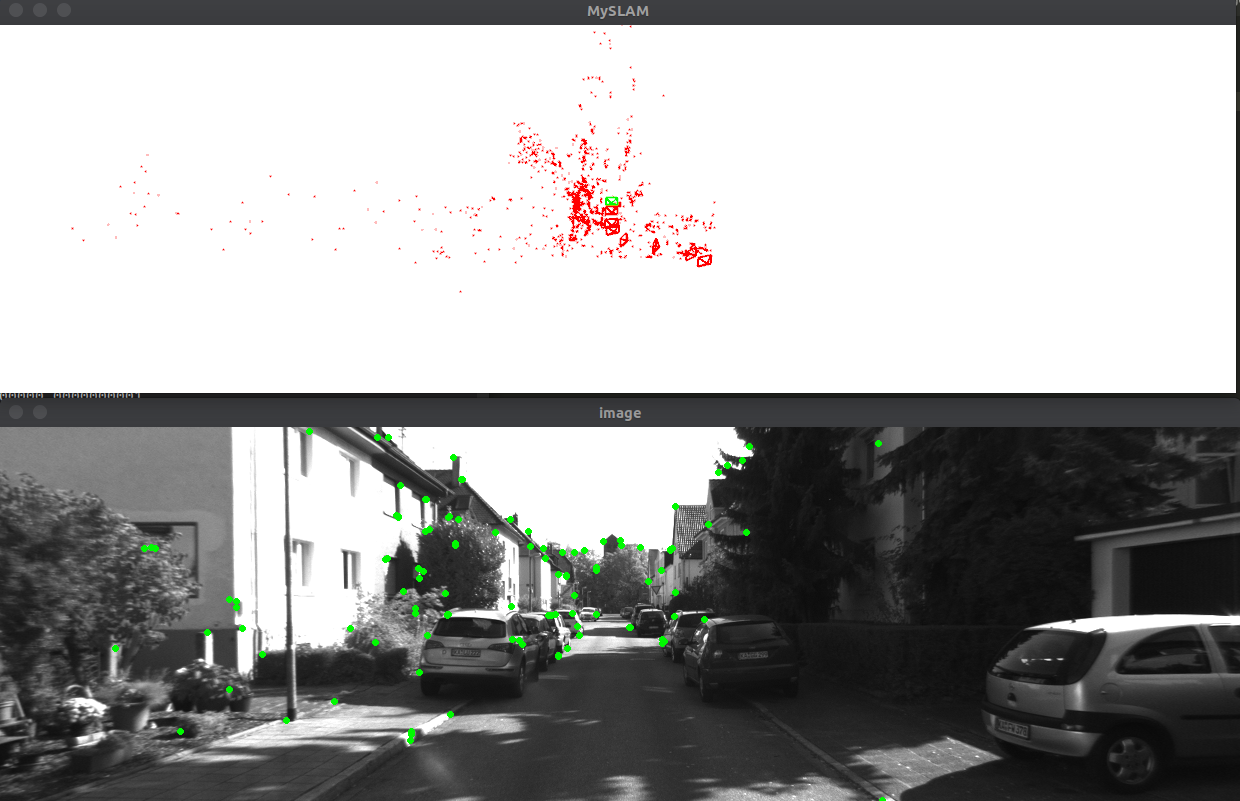
\includegraphics[width=0.9\linewidth]{designVO/snapshot-vo.png}\\
	\caption{Snapshot of the visual odometry.}
	\label{fig:snapshot-vo}
\end{figure}

We output the run time it takes for a single frame. When dealing with non-keyframes, the time is about 16ms. When processing keyframes, the time-consuming will increase due to the addition of a new step to extract feature points and find the right image matching. Moreover, since our map currently stores all keyframes and map points, it will cause memory growth after running for a period of time. If readers do not need all maps, they can keep only the active part.

\section*{Exercises}
\begin{enumerate}
	\item Do you understand all the C++ techniques used in this book? If there is something you are not familiar, use search engines to learn related knowledge, including: range-based for loops, smart pointers, singleton patterns in design patterns, and so on.
	\item Consider optimizing the system introduced in this lecture. For example, use a faster method of extracting feature points (this demo uses GFTT, which is not fast), use a 1-dimensional search instead of two-dimensional optical flow when matching left and right images, and use the direct method to estimate the pose and features at the same time, etc.
	\item* Add a loop detection thread to the demo, and use pose graph to optimize when a loop is detected to eliminate accumulated errors.
\end{enumerate}


